\chapter{Fundamentos tecnológicos}

El objetivo de este capítulo es presentar una introducción y unos fundamentos sobre la tecnología que da soporte a las organizaciones sobre las que se ejecutará el sistema recomendador, pues se considera que es importante entender sus limitaciones y el valor de estas tecnologías.

\section{Blockchain}

Un \textit{blockchain} (cadena de bloques) es un libro contable o \textit{ledger} distribuido que almacena una lista de transacciones. Cada bloque está firmado digitalmente utilizando los datos del bloque anterior, formando una cadena de tal manera que, de modificar un bloque, cambiaría la firma de todos los posteriores. Al estar esta lista distribuida, si uno de los nodos que almacena la lista cambia los datos, se produciría una incongruencia que sería detectada por el resto de nodos, por lo que podemos considerar el blockchain como una base de datos distribuida e inmutable, a la que solo se le pueden añadir datos.

Para realizar una nueva operación, el usuario utiliza una clave privada para firmar la transacción y la envía a algún nodo que participe en la red para que verifique la firma utilizando su clave pública, y se añada a la cadena. Sin embargo, los nodos que participan en la red necesitan de cierta comisión para realizar la operación. El \textit{hash} de la clave pública es la dirección que identifica al usuario, y que deberá usarse para realizar una transferencia. El programa o dispositivo que almacena esta clave privada se le conoce como cartera o \textit{wallet}, por lo que es común utilizar indistintamente este término para identificar a los usuarios. Nótese que al igual que en otras plataformas hay ciertos usuarios con varias cuentas, en blockchain también hay usuarios con varios \textit{wallets}, es decir, varias direcciones.

Tras procesar todas las transacciones realizadas desde el comienzo de la cadena de bloques, se obtiene el estado actual, con las cantidades obtenidas por cada usuario.

En 2008, una persona o grupo de personas conocido por el seudónimo de Satoshi Nakamoto desplegó satisfactoriamente Bitcoin, creando así la primera criptomoneda. Años después, en 2015 se lanzaría Ethereum~\cite{tual_ethereum_2015}, un blockchain desarrollado por el programador Vitalik Buterin que añadiría la revolucionaria capacidad de desplegar aplicaciones descentralizadas.

El conjunto de nodos participantes en la red de Ethereum forma una máquina virtual determinista basada en pila conocida como \gls{evm}. Esta máquina virtual ejecuta contratos inteligentes o \textit{smart contracts} que son desplegados por los usuarios. En este caso, una dirección de Ethereum puede representar tanto a un usuario como a un contrato inteligente, pero como estos últimos tienen las mismas capacidades que cualquier usuario, no se suele realizar ninguna distinción y se les considera simplemente otro tipo de agentes dentro del sistema.

Los contratos inteligentes se programan en un lenguaje de alto nivel y son compilados a \textit{bytecode} turing-completo del \gls{evm}, por lo que aunque su binario es público, el código fuente no lo es. Es común publicar el código fuente y las opciones del compilador utilizado para que los usuarios puedan verificar que compila al binario desplegado. Al igual que en Bitcoin, los usuarios deben pagar una comisión a los nodos para que su interacción con el contrato inteligente sea ejecutada.

Una de las mayores aplicaciones de este tipo de contratos es \gls{defi}, con la que se ofrecen diversos instrumentos financieros: préstamos, bonos, bolsas de valores, \textit{crowdfunding}... Sin embargo, las aplicaciones descentralizadas no se limitan sólo a las finanzas, también hay aplicaciones de juegos, energía, salud, ciencia, multimedia, entre otras~\cite{wu_first_2021}.

Para facilitar su uso, las aplicaciones descentralizadas utilizan una interfaz web a la que cualquiera puede acceder y leer los datos, aunque es necesario una extensión de navegador que haga de cartera para poder interactuar.

\section{Organizaciones Autónomas Descentralizadas}

Una \acrfull{dao} es un sistema basado en blockchain que permite a un grupo de personas coordinarse y auto-gobernarse mediante contratos inteligentes, y cuya gobernanza es descentralizada~\cite{hassan_decentralized_2021}. El término fue inventado en 2014 por Vitalik Buterin, programador de Ethereum~\cite{buterin_daos_2014}.

En la práctica, una \gls{dao} es un conjunto de contratos inteligentes que permiten a un conjunto de usuarios votar en propuestas, que tienen como efecto el realizar transacciones con su tesorería común, aceptar nuevos miembros, o incluso hacer llamadas a otros contratos inteligentes. En algunas organizaciones, es posible realizar propuestas aunque no se sea miembro, aunque sólo los miembros pueden votar.

Estas organizaciones han sido utilizadas para diversos propósitos, como votar propuestas de micromecenazgo y asignar presupuestos para invertir en la comunidad de manera participativa, similar a los presupuestos participativos. Además, existen organizaciones encargadas de administrar protocolos descentralizados, como las DAOs de Uniswap o Decentraland, así como de realizar compras de gran valor de manera conjunta, como el caso destacado de ConstitutionDAO, que recaudó 47 millones de dólares para adquirir una de las copias de la constitución estadounidense~\cite{kastrenakes_crypto_2021}. También se encuentran organizaciones más pequeñas que sirven para gestionar y administrar colectivos de desarrolladores o artistas, adoptando una estructura similar a la de una cooperativa~\cite{pena-calvin_categorization_2023}.

Debido a que es posible que una única persona tenga múltiples direcciones, en lugar de utilizar el esquema de un voto por persona, la organización asigna un \gls{vp} a cada usuario. La manera de asignar el \gls{vp} varía en cada comunidad, pero puede estar vinculado a la aportación de capital, a la realización de trabajos previos, o incluso ser asignada mediante propuestas de petición de \gls{vp}.

Debido a la inherente transparencia de Ethereum, el resultado de la votación y qué votó cada uno de los usuarios es siempre visible. Aunque podría ofuscarse o, incluso, encriptarse, las plataformas lo muestran sin ningún problema en la interfaz web.

Para evitar tener que programar una DAO desde cero, surgieron distintas plataformas para facilitar su despliegue a través de plantillas y sin necesidad de conocimientos de programación~\cite{faqir-rhazoui_comparative_2021}, dando lugar a un auge en la creación de organizaciones, llegando actualmente a registrarse más de 3 millones de miembros activos y manejando más de 30 mil millones de dólares estadounidenses en sus tesorerías, según el portal de analíticas Deepdao~\cite{deepdao_ventures_ltd_deepdao_2023}.

Aun así, las comunidades sufren de distintos problemas de seguridad, eficiencia, efectividad, y descentralización~\cite{buterin_governance_2018,buterin_moving_2021}, que intentan paliar utilizando métodos de votación distintos a la mayoría absoluta o relativa~\cite{fan_insight_2023}. Estos sistemas pueden llegar a ser muy complejos y difíciles de comprender por los usuarios, dificultando la participación.

Algunas comunidades intentan paliar estas cuestiones con medios externos a la blockchain. Por ejemplo, una práctica común es discutir minuciosamente una propuesta en foros o chats antes de subir la propuesta formalmente a la plataforma, asegurándose así de que será aprobada. Sin embargo, se reduce la transparencia del sistema pues no toda la comunidad participa en dichos canales, y algunos de ellos son jardines vallados a los que es imposible acceder sin registro previo, dependientes de una entidad central. Otros sistemas de votación permiten \textit{delegar} tu poder de votación, confiando en el juicio de individuos de confianza. En ambos casos, es necesario que al menos un usuario asuma la responsabilidad de estar al tanto de todas las propuestas, filtrarlas, y difundir su información o actuar de manera congruente. La ausencia de este usuario en momentos críticos de votación, o su decisión de modificar radicalmente su postura, podría desencadenar consecuencias adversas para la organización. Por ejemplo, si se lleva a cabo una votación para remunerar a un individuo que ha contribuido a la DAO, y dicha propuesta no obtiene aprobación, la confianza de otros colaboradores puede disminuir, desincentivando futuras colaboraciones.

Para mejorar la participación y disminuir los efectos del precio de Ethereum en la comunidad~\cite{faqir-rhazoui_effect_2021}, se ha buscado utilizar cadenas alternativas compatibles con la \gls{evm} y, por lo tanto, compatibles con el código de los contratos inteligentes desarrollados previamente. Estas cadenas suelen tener unos costes de operación menores, y un tiempo de bloque menor (es decir, tarda menos en ejecutarse cada operación), o están basadas en criptomonedas con precios estables, mejorando notablemente la usabilidad y obteniendo una rápida adopción.

\begin{figure}[t]
    \centering
    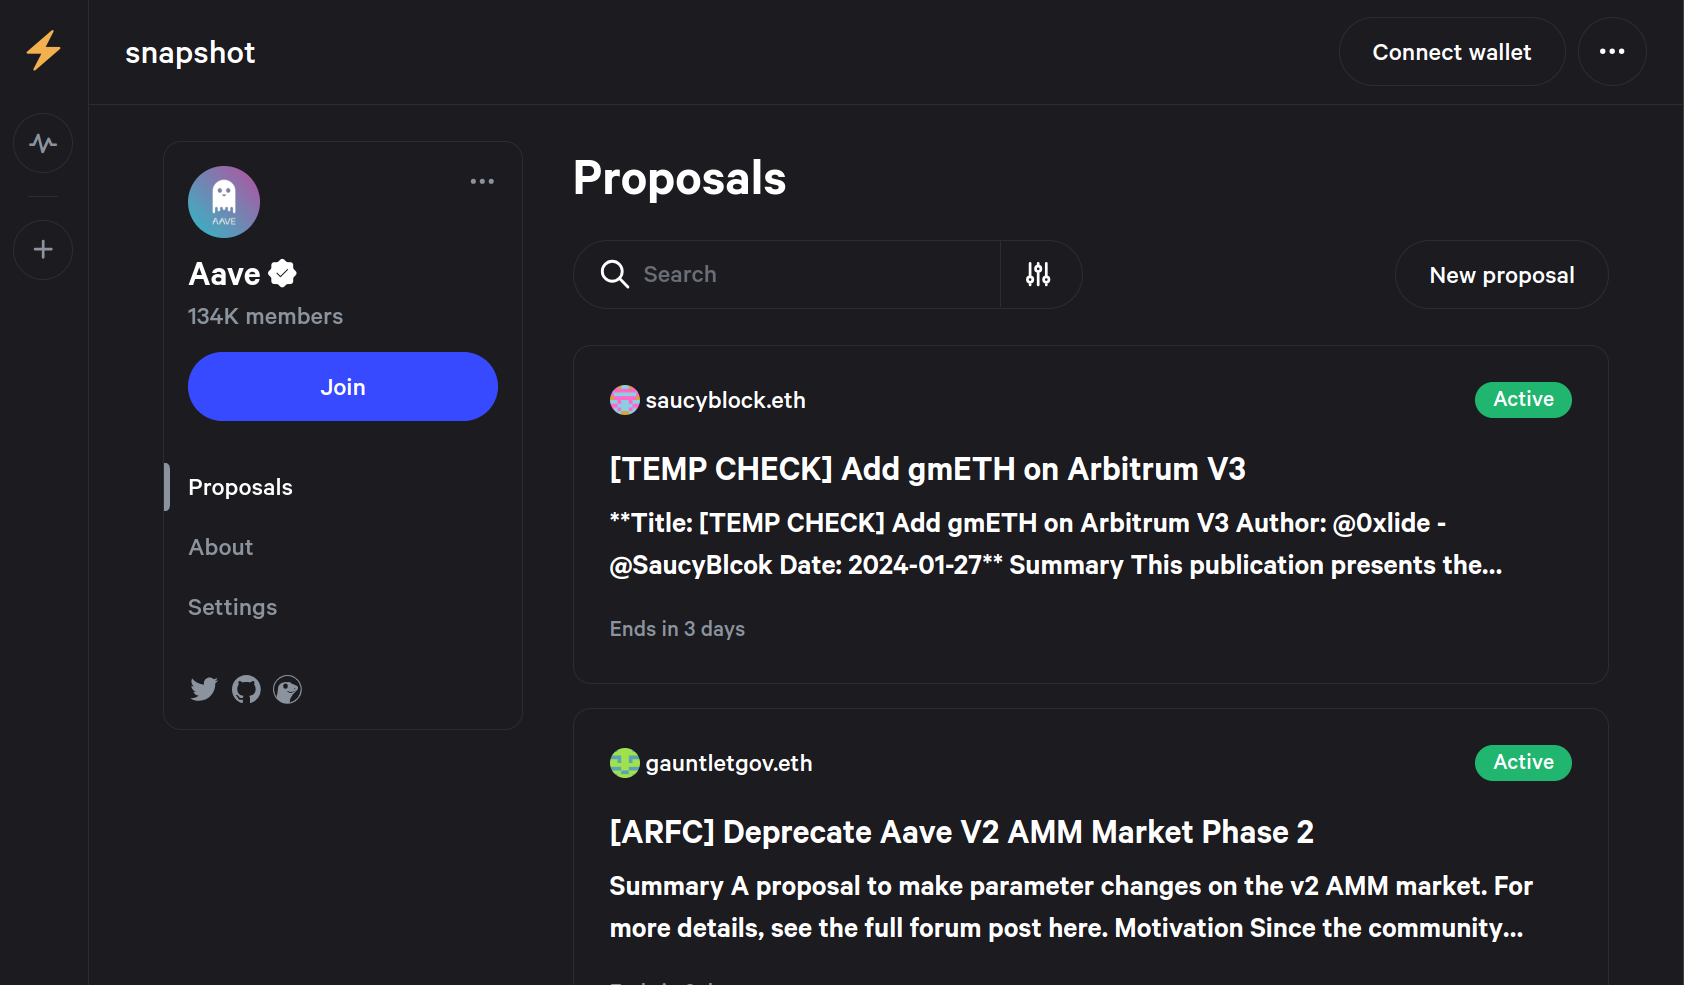
\includegraphics[width=\linewidth]{figures/02_sota/brave_screenshot_snapshot.org_aave.png}
    \setcaptionsource{\url{https://snapshot.org/\#/aave.eth}}
    \caption{Captura de pantalla de la interfaz web de la plataforma Snapshot para la gobernanza de la organización Aave.}
    \label{fig:screenshot_snapshot-gui}
\end{figure}

Finalmente, en 2021 se lanzó la plataforma \textit{off-chain} y, por lo tanto, sin costes de operación, pero manteniendo la seguridad y descentralización necesarias para las DAOs llamada Snapshot. Para mantener la descentralización, los votos están firmados digitalmente usando la clave privada del usuario, y tanto la interfaz como los resultados son almacenados en \gls{ipfs}, un protocolo de hipertexto descentralizado. Sigue teniendo las mismas capacidades de conectarse con una tesorería, realizar transferencias y ejecutar cualquier contrato inteligente, por lo que a efectos prácticos es como una DAO sin blockchain y mejor usabilidad. En la figura~\ref{fig:screenshot_snapshot-gui} se muestra una captura de la interfaz web.

Esta plataforma elevó en varios órdenes de magnitud el alcance de las DAOs, alojando actualmente más de 30 mil organizaciones que suman más de 3 millones de usuarios y 200 mil propuestas realizadas~\cite{pena-calvin_census_2024}.
